\documentclass[H1,manyauthors]{ALICE_analysis_notes}
%\documentclass[ALICE,manyauthors]{ALICE_scientific_notes}
%

\usepackage{cite}
\usepackage[toc,page]{appendix}

\newcommand{\pt}{\ensuremath{p_{\mathrm{T}}}}
\newcommand{\ptreco}{\ensuremath{p_{\mathrm{T}}^{\mathrm{reco}}}}
\newcommand{\pttruth}{\ensuremath{p_{\mathrm{T}}^{\mathrm{true}}}}
\newcommand{\pttrack}{\ensuremath{p_{\mathrm{T}}^{\mathrm{track}}}}
\newcommand{\ptjet}{\ensuremath{p_{\mathrm{T}}^{\mathrm{jet}}}}
\newcommand{\ptgamma}{\ensuremath{p_{\mathrm{T}}^{\mathrm{\gammaiso}}}}
\newcommand{\ptcluster}{\ensuremath{p_{\mathrm{T}}^{\mathrm{cluster}}}}


\newcommand{\etajetlab}{\ensuremath{\eta_{\mathrm{lab}}^{\mathrm{jet}}}}


\newcommand{\slfrac}[2]{\left.#1\right/#2}
\usepackage{rotating}
\usepackage{placeins}
\usepackage{algpseudocode}
\usepackage{graphicx}
%\usepackage{subcaption}
\usepackage{lipsum}
\usepackage{lineno}
\usepackage[colorlinks=true,citecolor=blue]{hyperref}
\usepackage{multirow}
%\usepackage{authblk}

\usepackage{textcomp}
%\usepackage{lmodern}  % for bold teletype font
\usepackage{amsmath}  % for \hookrightarrow
\usepackage{xcolor}   % for \textcolor
\usepackage{listings}
\lstset{
  basicstyle=\ttfamily,
  columns=fullflexible,
  frame=single,
  breaklines=true,
  postbreak=\mbox{\textcolor{red}{$\hookrightarrow$}\space},
}

\linenumbers
\begin{document}%
%%%%%%%%%%%%% ptdr definitions %%%%%%%%%%%%%%%%%%%%%
%
%%%%%%%%%%%%%%%  Title page %%%%%%%%%%%%%%%%%%%%%%%%
%
\begin{titlepage}
%
\PHnumber{v1.0}
\PHdate{\today}
%
%%% Put your own title + short title here:
\title{Long-range azimuthal di-hadron correlations with CLAS12}
\ShortTitle{Long-range azimuthal di-hadron correlations with CLAS12}   % appears on right page headers
%


\author{Sebouh Paul and Miguel Arratia}



%
\begin{abstract}
We present a study of long-range azimuthal dihadron correlations with CLAS12. 
\end{abstract}
\end{titlepage}
\tableofcontents
\section{Introduction}

\section{Data and MC sets}
\label{data}
We used the in-bending RGA data from the fall 2018 run period.  The files can be found in

/lustre/expphy/cache/clas12/rg-a/production/recon/fall2018/torus-1/pass1/v0/dst/

For the Monte-Carlo simulations, we used the corresponding no-background DIS simulations located at:

/work/clas12/rg-a/montecarlo/fall2018/torus-1/clasdis/nobg/
\section{Event Selection} \label{sec:eventselection}
The first step in the analysis is creating tuples in ROOT, which use the event selection criteria in Secs.~\ref{sec:electron_selection} and 
\label{sec:hadron_selection}, which follow \cite{RGANote}.  Further analysis cuts are described in Sec.~\ref{sec:analysis_selection}.
\subsection{Electron Selection}
\label{sec:electron_selection}
The electron identification uses the following cuts:

\begin{itemize}
    \item The EC fraction, $E_{\rm EC}/p$, is at least 0.17
    \item The energy measured in the PCAL is at least 0.07 GeV
    \item The vertex position is between $-$13 and 12 mm ($-$18 and 10 mm) for data with in-bending (out-bending) torus field.  
    \item The tracks are in the fiducial part of the drift chamber and the PCAL, as described in \cite{RGANote}.  
    \item The particle's charge is negative.
\end{itemize}


In order to select deep-inelastic-scattering (DIS) events, we require the following kinematic cuts:
\begin{itemize}
    %\renewcommand\labelitemi{$\bullet$}
    \item four-momentum transfer: $Q^2>1$ GeV$^2/c^2$
    \item hadronic-system mass: $W>2$ GeV$/c^2$
    \item energy loss fraction: $y_e\equiv \nu/E<0.85$
\end{itemize}

\subsection{Hadron selection}
\label{sec:hadron_selection}
To identify hadrons, we use the following cuts:
\begin{itemize}
    %\renewcommand\labelitemi{$\bullet$}
    \item Goodness of pid: |\texttt{chi2pid}|$<3\sigma$, where $\sigma$ is determined for $\pi^+$ and $\pi^-$ in \cite{RGANote}.  For $p$, we used $\sigma=1.3$.  For the $\pi^\pm$ we used tightened cuts for positive \texttt{chi2pid} following \cite{RGANote} to reduce contamination from kaons.
    \item The difference in vertex positions in $z$ between the hadron candidate and the electron is less than 20 mm.  
    \item The difference in time between the electron and the hadron candidate (after subtracting the pathlength divided by the velocity calculated using the momentum and the PDG mass of the particle) is less than 0.3 ns
    \item The particle is in the fiducial part of the drift chamber.  
\end{itemize}

\subsection{Analysis selection cuts}
\label{sec:analysis_selection}
In addition to the tuple creation criteria, we make the following analysis cuts:
\begin{itemize}
    \item For $\pi p$ events, we require the missing mass $m_{X}(ep\rightarrow eh_1X)$ to be at least 1.665 GeV.  This avoids events where the proton is a decay product of a $\Delta$ resonance, the mass of which is 1.232 GeV$/c^2$.  This cut is chosen to be approximately 3 sigma above the resonance mass.  
\end{itemize}
\section{Data/MC comparison and MC re-weighting}\label{sec:dataMCcomparison}


\section{Extraction of correlation functions and analysis}\label{sec:corr}
To extract the correlation functions, we first obtain the same-event yields as a function of $\Delta \phi$ and $\Delta y$, defined as 
\begin{equation}
    S(\Delta\phi,\Delta y) = \frac{1}{N_{\rm trig}}\frac{dN^{\rm same}}{d\Delta \phi d\Delta y}
\end{equation}
where $N_{\rm trig}$ is the number of trigger hadrons in the event sample\footnote{This includes those without an associated hadron.  Therefore the integral of $S(\Delta\phi,\Delta y)$ is not necessarily 1, but rather the ratio of the number of associated hadrons in events with a trigger hadron in the event sample to the number of trigger hadrons.}.
Then we obtain the normalized mixed yield, defined as
\begin{equation}
    M(\Delta\phi,\Delta y) = \frac{1}{N^{\rm mix}_{\rm tot}}\frac{dN^{\rm mix}}{d\Delta \phi d\Delta y}(\Delta \phi,\Delta y)
\end{equation}
The correlation function, which is expected to be free of detector effects, is defined as 
\begin{equation}
    C(\Delta\phi,\Delta y) = \frac{S(\Delta\phi,\Delta y)}{M(\Delta\phi,\Delta y)}.
\end{equation}

For the 1D projection $C(\Delta\phi)$ for large rapidity separation, we take the ratios of the the integrals of both the same- and mixed-event yields:
\begin{equation}
    C(\Delta\phi) = \frac{\int_{\Delta y_{\rm min}}^{\Delta y_{\rm max}} d\Delta y  [S(\Delta\phi,\Delta y)]}{\int_{\Delta y_{\rm min}}^{\Delta y_{\rm max}} d\Delta y [M(\Delta\phi,\Delta y)]},
\end{equation}
where we choose $\Delta y_{\rm min}$ and $\Delta y_{\rm min}$ to be 1.5 and 2.5 respectively for this analysis.  
\subsection{Fourier analysis}
\label{sec:fourier}
Fourier transforms are performed on the correlation function $C(\Delta\phi)$.  In principle the coefficients $V_n$ may be compared to predictions made using structure functions.  

\begin{equation}
    f(\Delta\phi) = A(1+2\sum\limits_n V_n\cos (n\Delta\phi))
\end{equation}

\subsection{Ridge yield}
Some theoretical models predict the existence of a bump in the correlation function at $\Delta\phi=0$ [insert reference].  These have been observed in large multiplicity events at CMS in PbPb, $p$Pb, and $pp$  scattering reactions \cite{Khachatryan:2010gv,CMS:2012qk,Khachatryan:2015lva}.  In addition, limits have been set in ALEPH \cite{Lee:2019tmr} and preliminary results from HERA [insert citation] 

Following [insert citation], we use the zero-yield at minimum (ZYAM) procedure to determine the ridge yield, as illustrated in Fig.~\ref{fig:ridge_yield_procedure}.   The first step is fitting the correlation function to a 3rd order Fourier series $f(\Delta\phi)$ (see Sec.~\ref{sec:fourier}.  If the fit function is concave-up at $\Delta\phi=0$, then the yield is zero.  Otherwise, if $f''(0)$ is negative, then the minimum of the function is found, where $f'(\Delta\phi_{\rm min})=0$.  The value of the fit at the minimum is then subtracted from the total correlation function, and then the integral of the correlation function is between $-\Delta\phi_{\rm min}$ and $\Delta\phi_{\rm min}$ is found.  This is then normalized by dividing it by the integral of the correlation function (pre-subtraction) over the full $-\pi$ to $\pi$ range. 

In order to determine upper limits on the ridge yield, we perform a bootstrap procedure \cite{10.1214/aos/1176344552}, in which the values in each bin are randomly modified by a gaussian whose mean is equal to the measured value in the bin, and the sigma is the statistical uncertainty in that bin.  The ridge-yield analysis procedure is repeated on each bootstrap iteration XXXX times, and the upper limits are obtained as the 95th percentile of the yields for the bootstraps.  

\begin{figure}
    \centering
    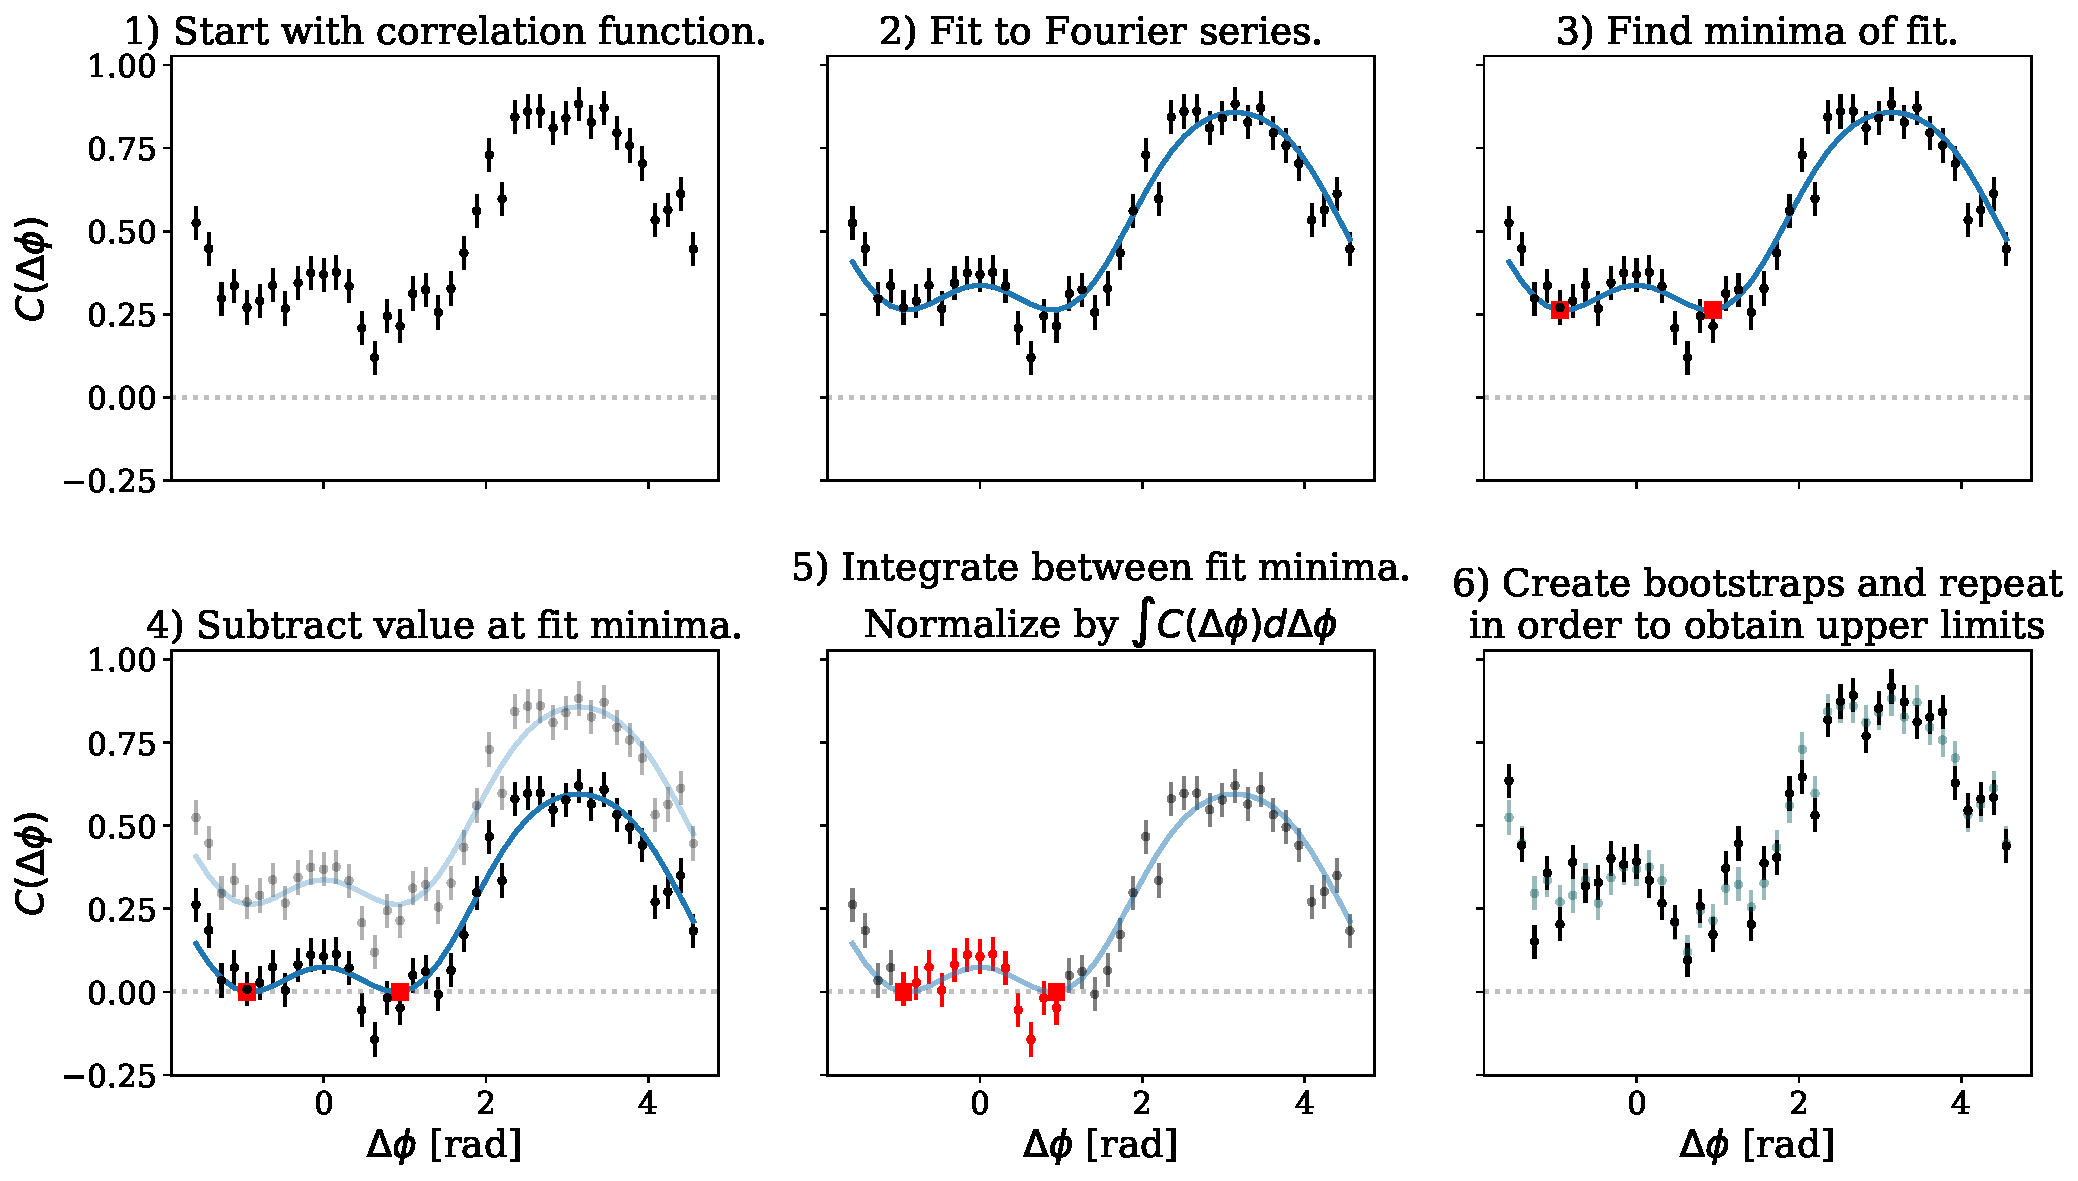
\includegraphics[width=\textwidth]{ridge_yield_procedure.pdf}
    \caption{Illustration of ridge yield procedure}
    \label{fig:ridge_yield_procedure}
\end{figure}


%We took the Fourier transform of the correlation function $C(\Delta\phi)$.  Of particular interest is the parameter $v_2$, defined as the ratio of the $\cos 2\Delta\phi$ coefficient in the Fourier series of the correlation function to that of the constant term.
\section{Event Mixing}
The mixed event sample was produced combining the electron and pion in a ``trigger'' event with a hadron from another event (the ``associated'' event).  Both the trigger event and the associated event were required to have a DIS electron and a hadron which satisfy the requirements in Sec.~\ref{sec:eventselection}.  For the trigger event, the hadron was required to be a pion with at least $z>0.4$. However, neither the trigger event nor the associated event were required to have more than one hadron.  


All kinematic variables that depend on the associated hadron's kinematics and also the kinematics of the electron and/or trigger pion were recalculated using the kinematics of the associated hadron of the associated event and the electron and trigger pion of the trigger event.  Such variables include $z_2$, $\phi^{\rm cm}_2$, $\Delta\phi_{\rm cm}$, $m_{\rm pair}$, etc.  




\input{Systematics}
\section{Validation}
\subsection{Comparison of inbending and outbending data}
One of the validation tests performed on our data is to see if the results are independent of the torus-field polarity.  The first stage of this test is to select only events in the region of overlap between the two configurations.  For the data with the in-bending (out-bending) configuration, particles with positive (negative) charge can be observed at smaller polar angles\footnote{at the interaction point} than in out-bending (in-bending) configuration.  This is demonstrated in Figs.~\ref{fig:p_vs_th_inout_e}, \ref{fig:p_vs_th_inout_h1} and \ref{fig:p_vs_th_inout_h2}, which contain $p$ vs $\theta$ scatter plots of the in-bending (blue) and out-bending (orange) datasets (respectively  for $e$,$h_1$ and $h_2$).  Each of the panels shows a different configuration of hadron types.    

\begin{figure}
    \centering
    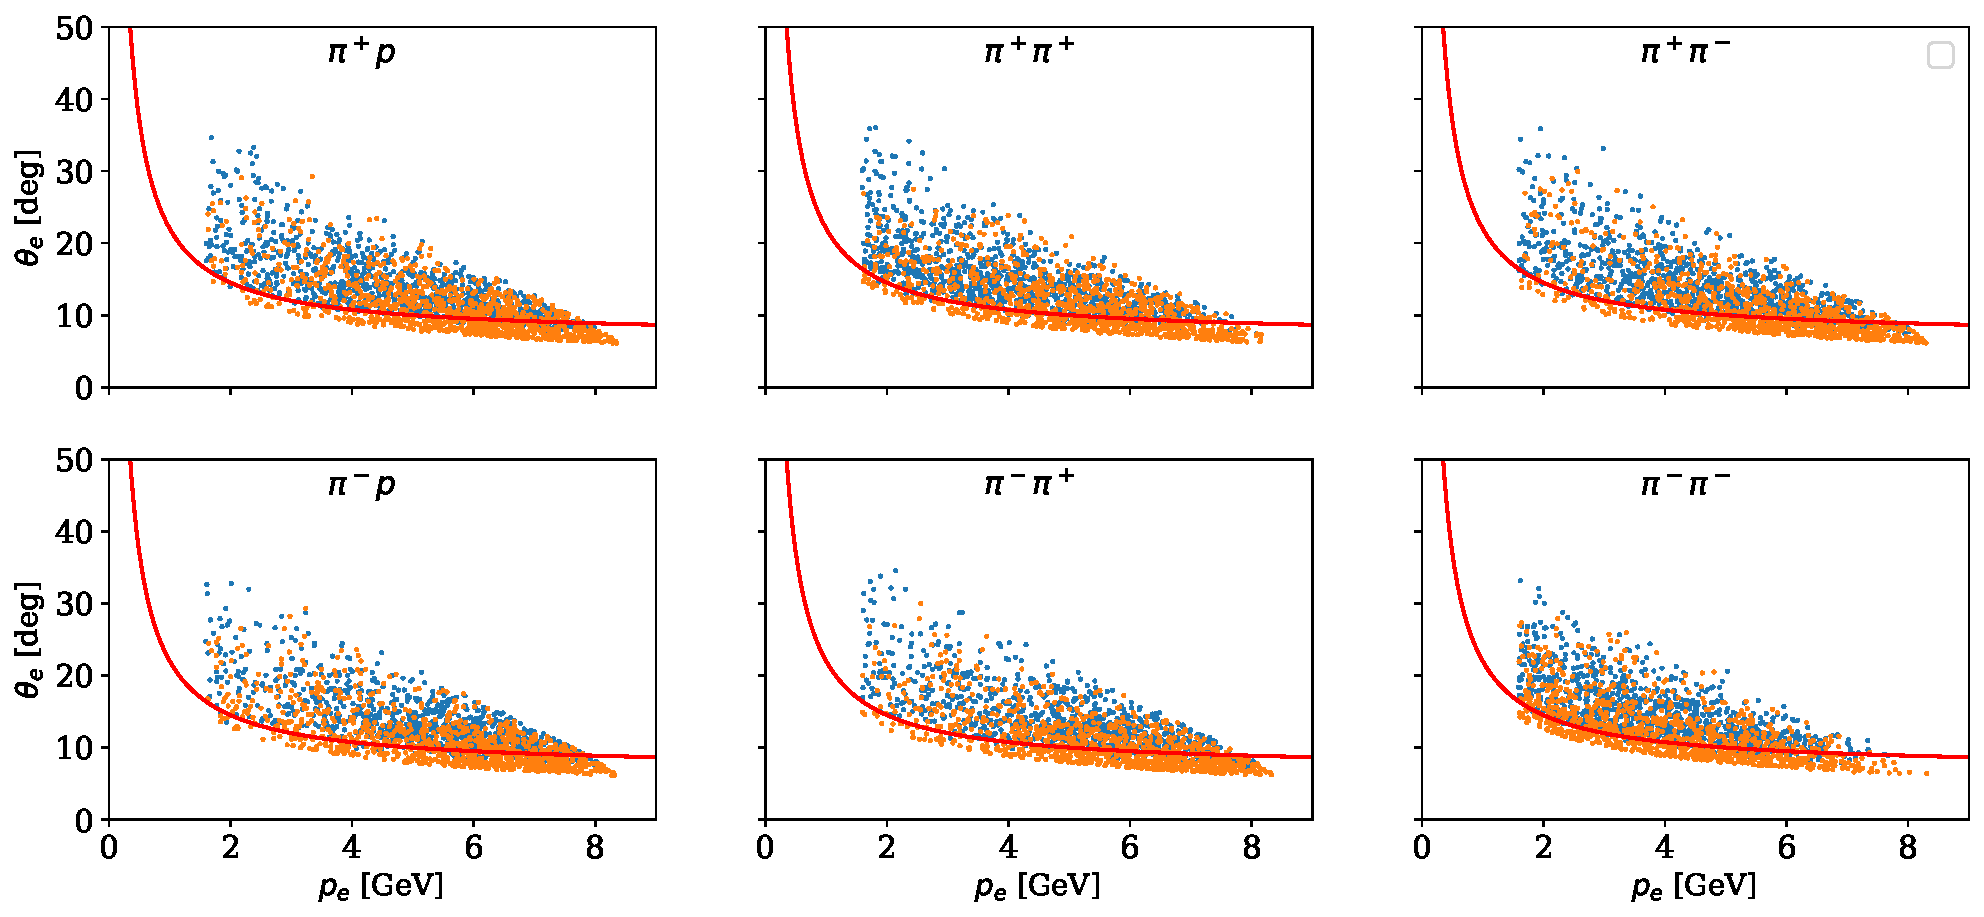
\includegraphics[width=\textwidth]{p_vs_th_inout_e}
    \caption{Electron momentum vs polar angle spectra (lab frame) for data in the in-bending (blue) and out-bending (orange) torus configurations.  The different panels represent different configurations of  di-hadron types.}
    \label{fig:p_vs_th_inout_e}
\end{figure}

\begin{figure}
    \centering
    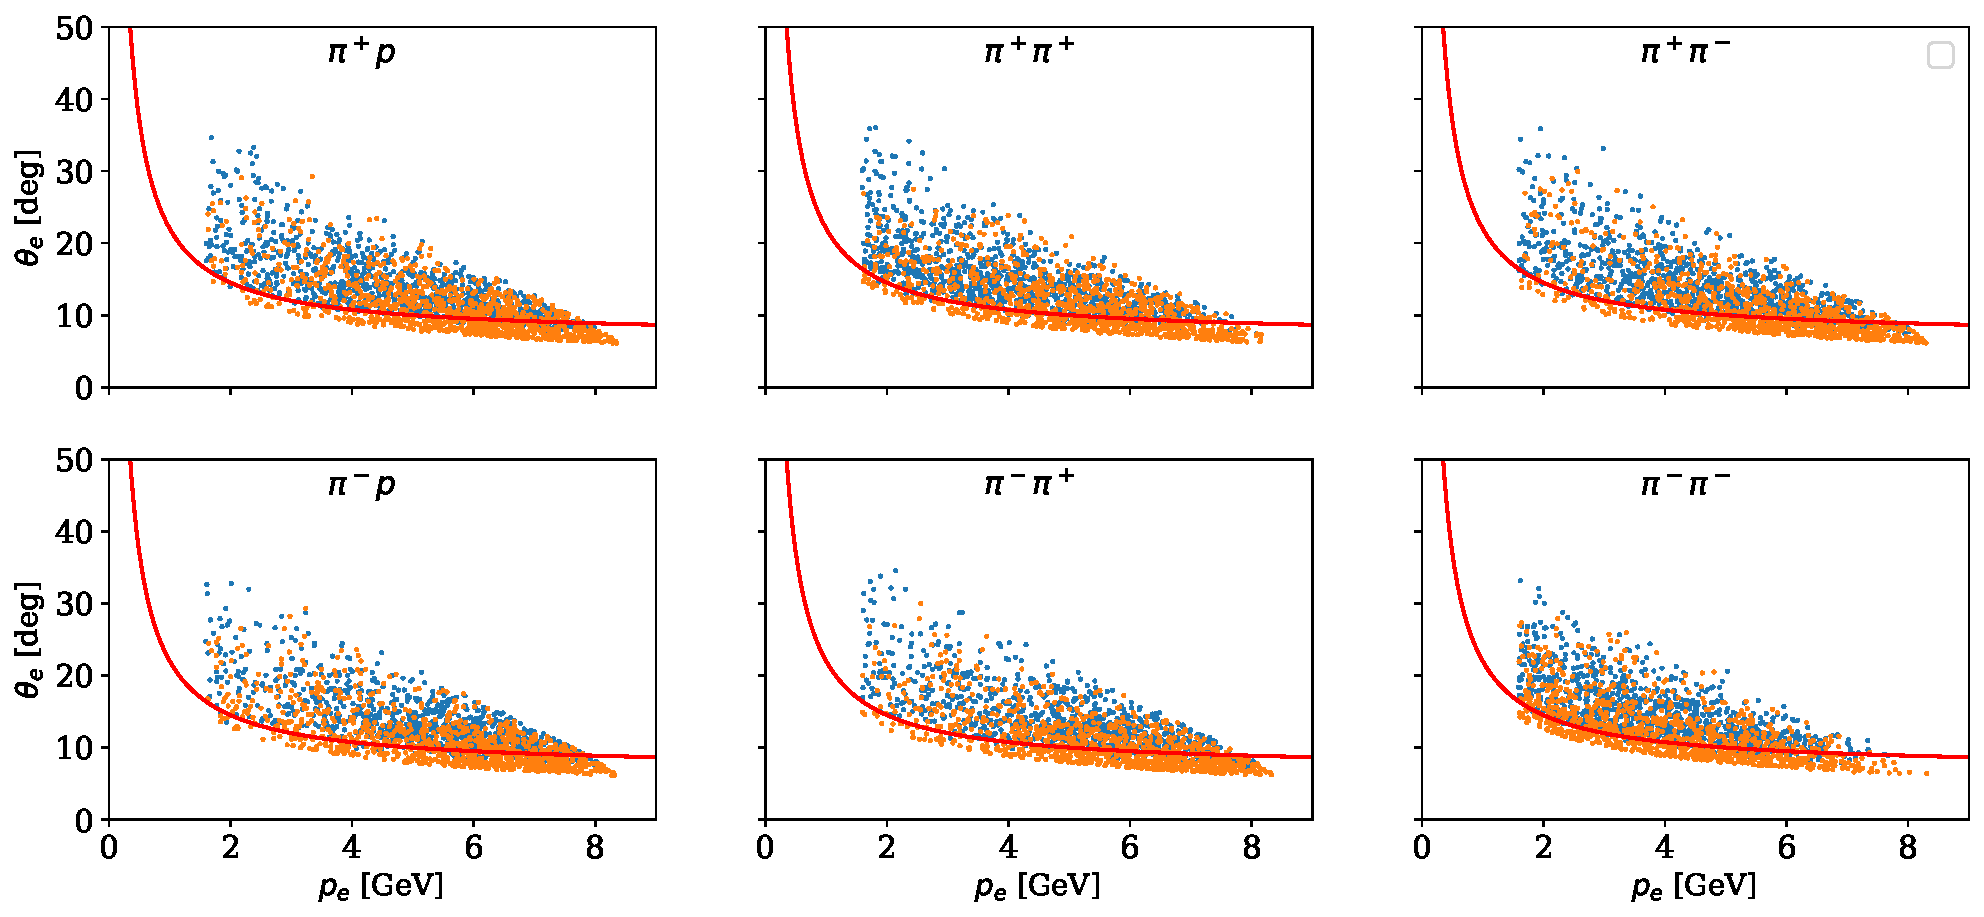
\includegraphics[width=\textwidth]{p_vs_th_inout_e}
    \caption{Same as \ref{fig:p_vs_th_inout_e} for the leading hadron's momentum and polar angle}
    \label{fig:p_vs_th_inout_h1}
\end{figure}

\begin{figure}
    \centering
    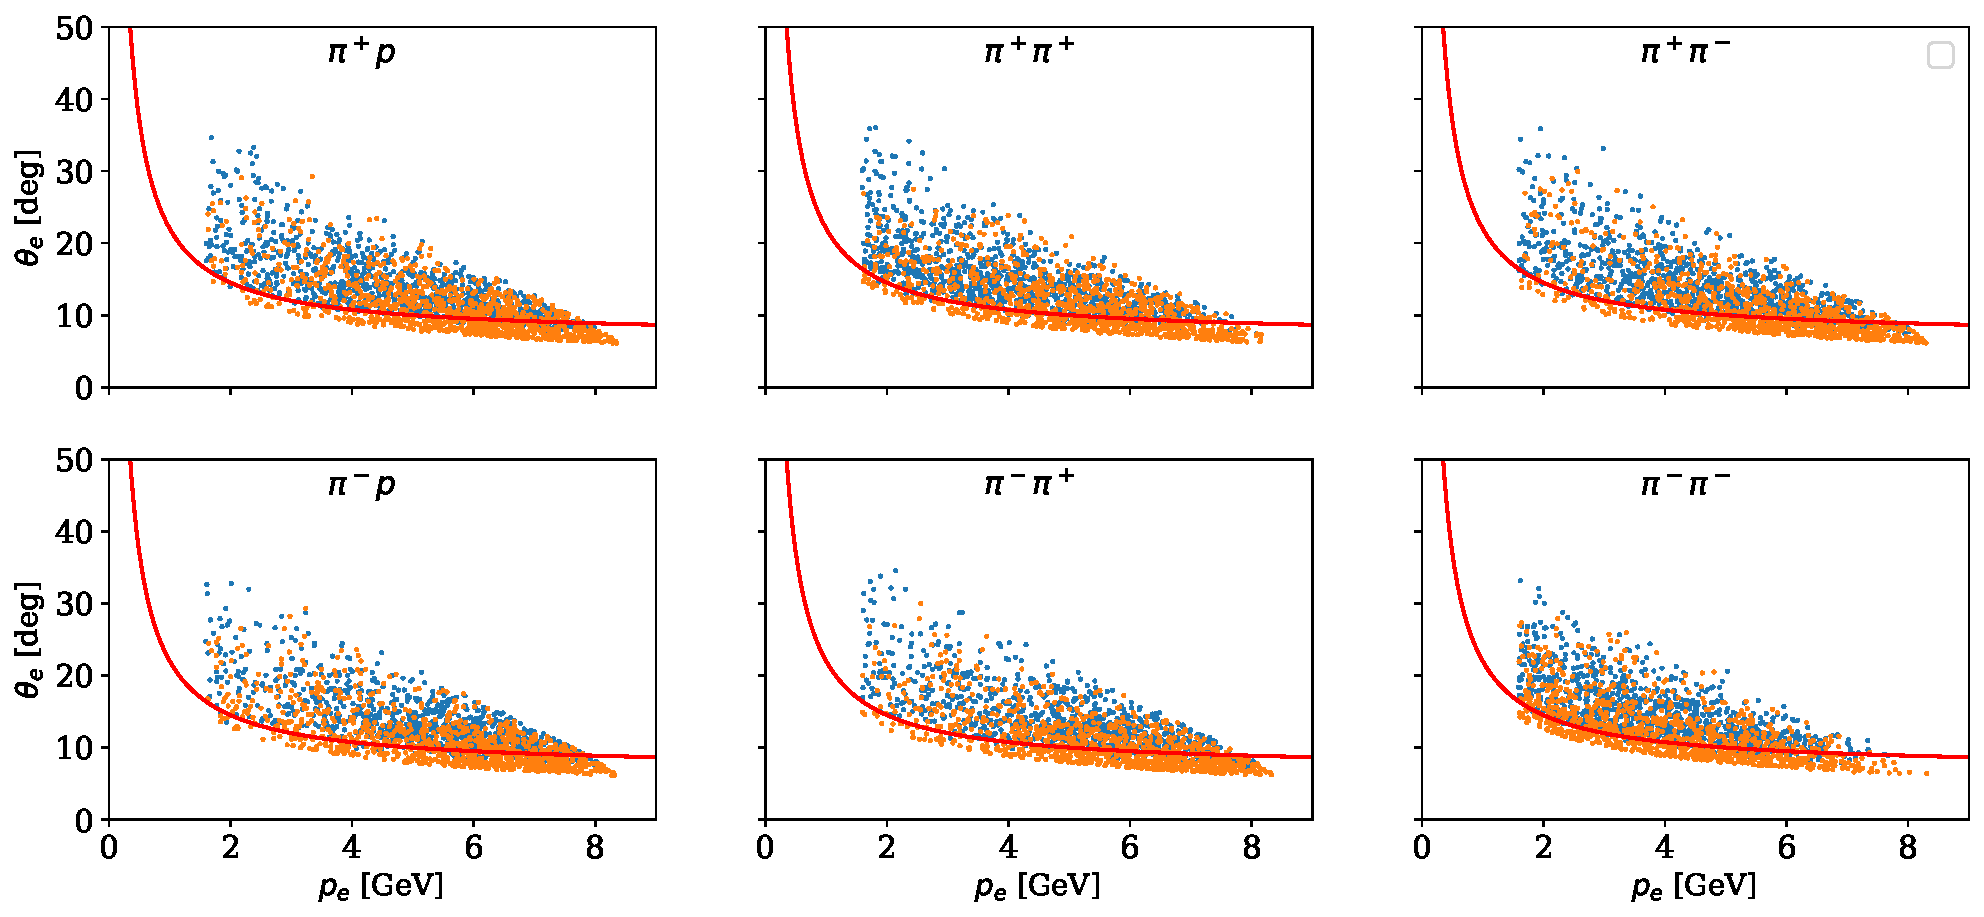
\includegraphics[width=\textwidth]{p_vs_th_inout_e}
    \caption{Same as \ref{fig:p_vs_th_inout_e} for the sub-leading hadron's momentum and polar angle}
    \label{fig:p_vs_th_inout_h2}
\end{figure}

In order to only include events in the kinematic region where the data taken with the two field polarities overlap, we used following kinematic cuts on each of the three particles ($e$,$h_1$ and $h_2$):
\begin{equation}
    \theta > 7\degree + \frac{15\degree}{p/{\rm GeV}}
\end{equation}
where $p$ and $\theta$ are the lab-frame momenta and polar angles for the particle.  This is shown as a red line in Figs.~\ref{fig:p_vs_th_inout_e}-\ref{fig:p_vs_th_inout_h2}.  



Figs.~\ref{fig:smc_pi+p_inout} through~\ref{fig:smc_pi+p-_inout} shows the same-event yields, mixed-event yields and correlation functions for each combination of particle observed ($\pi^+ p$, $\pi^- p$, $\pi^+\pi^+$, $\pi^-\pi^+$, and $\pi^+\pi^-$), with the exception of $\pi^-\pi^-$, for which we have very limited statistics. The top (bottom) panel of each figure shows the 2d functions for in-bending (out-bending) data.  The bottom panels show the 1d projections in the $\Delta y=1.5$ to 2.5 range, with in-bending (out-bending) data in blue (orange).  
\section{Results} \label{sec:results}

Figure~\ref{fig:corr_pi_p} shows the same-event yield (left panel), mixed event yield (middle panel) and correlation functions (right panels) as 2D functions of $\Delta\phi$ and $\Delta y$ (top) and 1D functions of $\Delta\phi$  for the $1.5<\Delta y<2.5$ region (bottom) for all $\pi p$ events.  The same types of plots are shown for $\pi^+p$, $\pi^-p$, and $\pi\pi$ events in Figs.~\ref{fig:corr_pi+_p} through \ref{fig:corr_pi_pi}

\begin{figure}
    \centering
    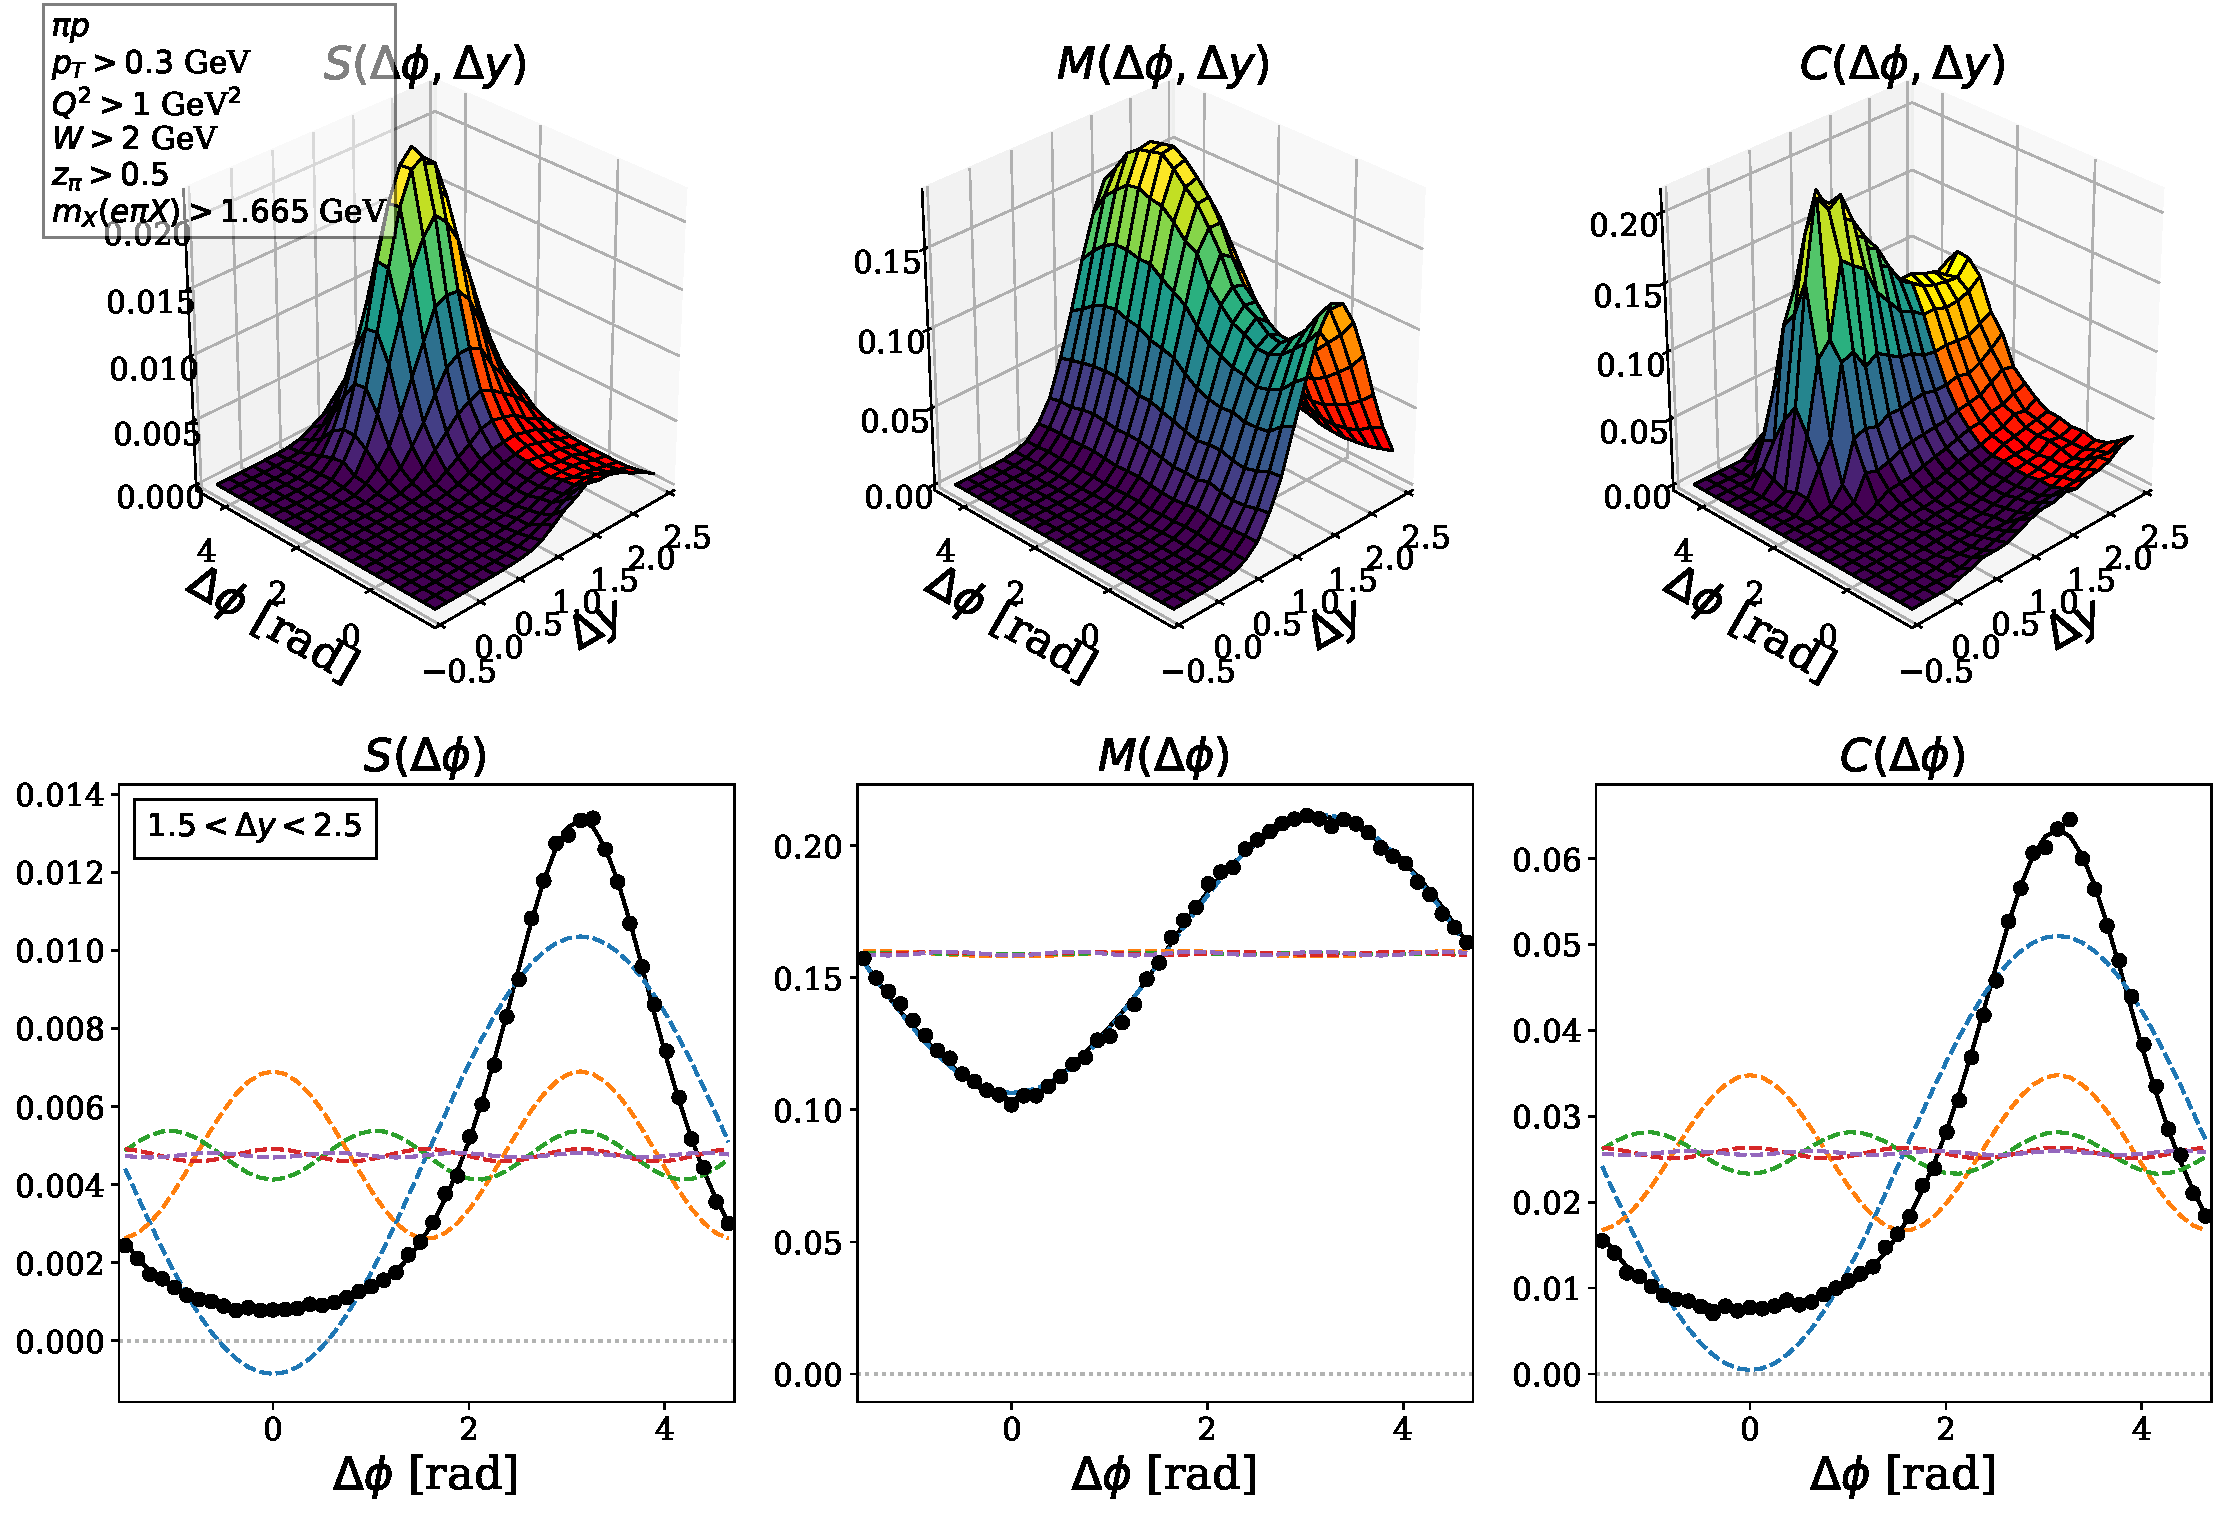
\includegraphics[width=\textwidth]{smc_pi_p.pdf}
    \caption{same-event yield (left panel), mixed event yield (middle panel) and correlation functions (right panels) as 2D functions of $\Delta\phi$ and $\Delta y$ (top) and 1D functions of $\Delta\phi$  for the $1.5<\Delta y<2.5$ region (bottom) for all $\pi p$ events.  The $1.5<\Delta y<2.5$ region is highlighted in the top row of plots using a brighter color scheme than the rest of the plot.}
    \label{fig:corr_pi_p}
\end{figure}

% \begin{figure}
%     \centering
%     \includegraphics[width=\textwidth]{dphi_vs_deta_pi+_p.pdf}
%     \caption{Same as Fig.~\ref{fig:corr_pi_p} for $\pi^+ p$ events.}
%     \label{fig:corr_pi+_p}
% \end{figure}

% \begin{figure}
%     \centering
%     \includegraphics[width=\textwidth]{dphi_vs_deta_pi-_p.pdf}
%     \caption{Same as Fig.~\ref{fig:corr_pi_p} for $\pi^- p$ events.}
%     \label{fig:corr_pi-_p}
% \end{figure}

\begin{figure}
    \centering
    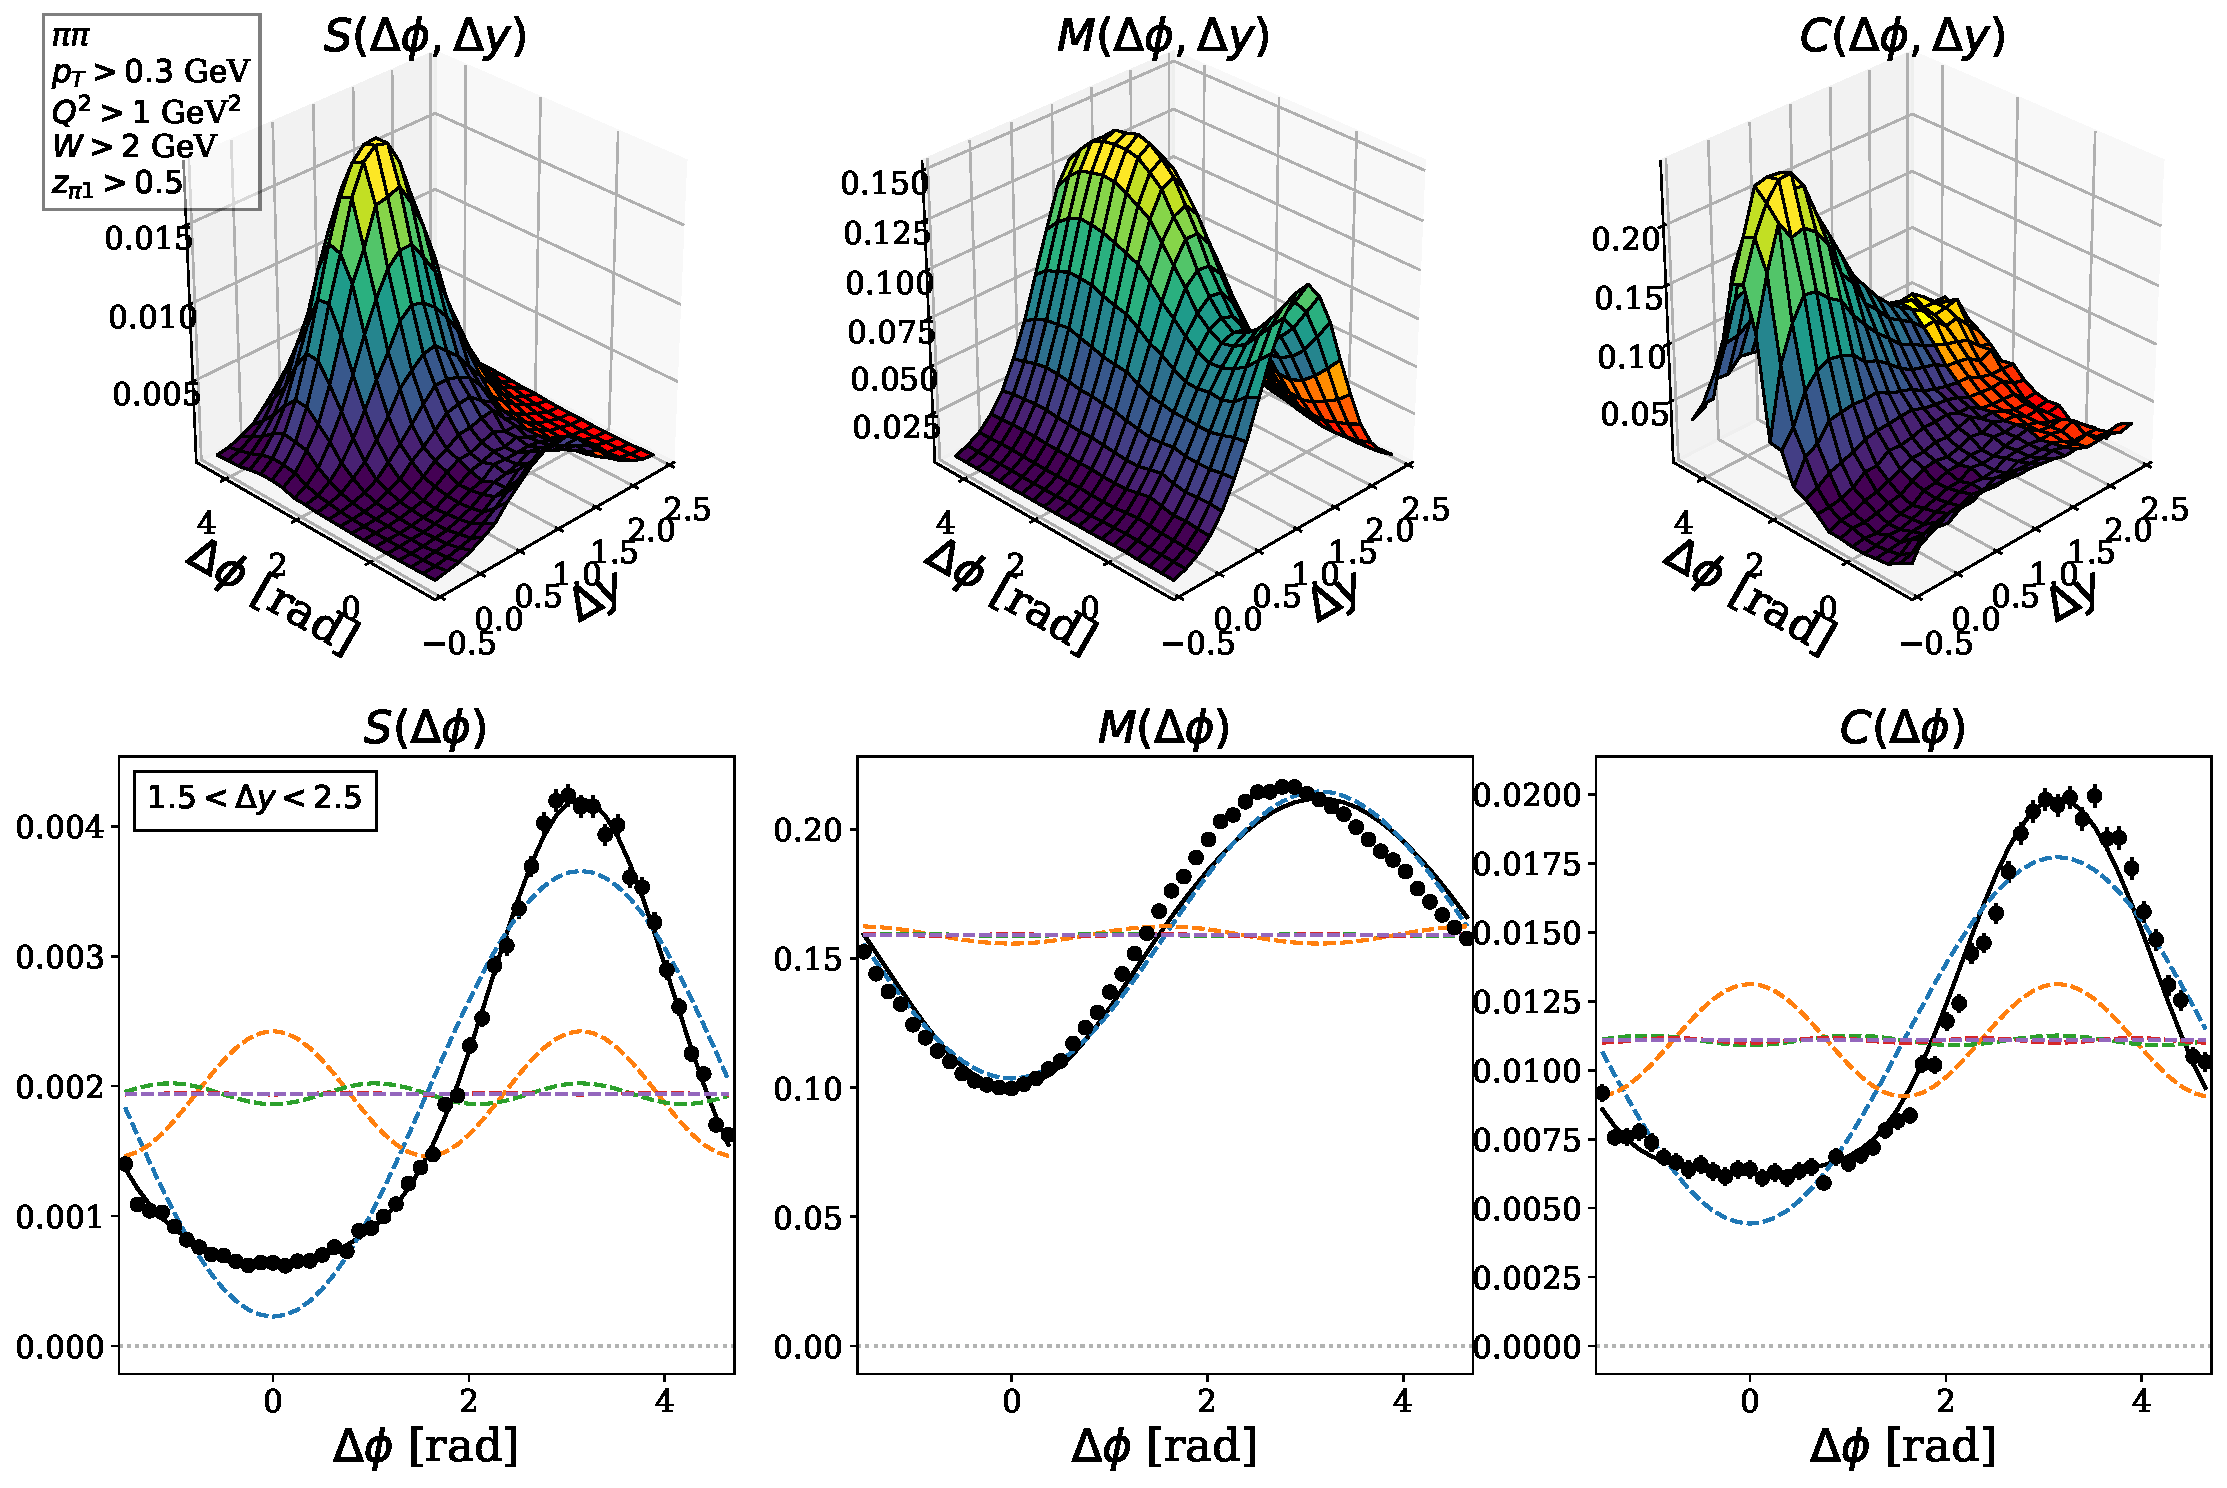
\includegraphics[width=\textwidth]{smc_pi_pi.pdf}
    \caption{Same as Fig.~\ref{fig:corr_pi_p} for $\pi\pi$ events.}
    \label{fig:corr_pi_pi}
\end{figure}

The values of $v_2$ are shown as functions of several kinematic variables in Fig.~\ref{fig:v2_vs_stuff}.  This quantity increases with larger $p_t$ of both hadrons, but it has very little dependance on the $Q^2$.  

\begin{figure}
    \centering
    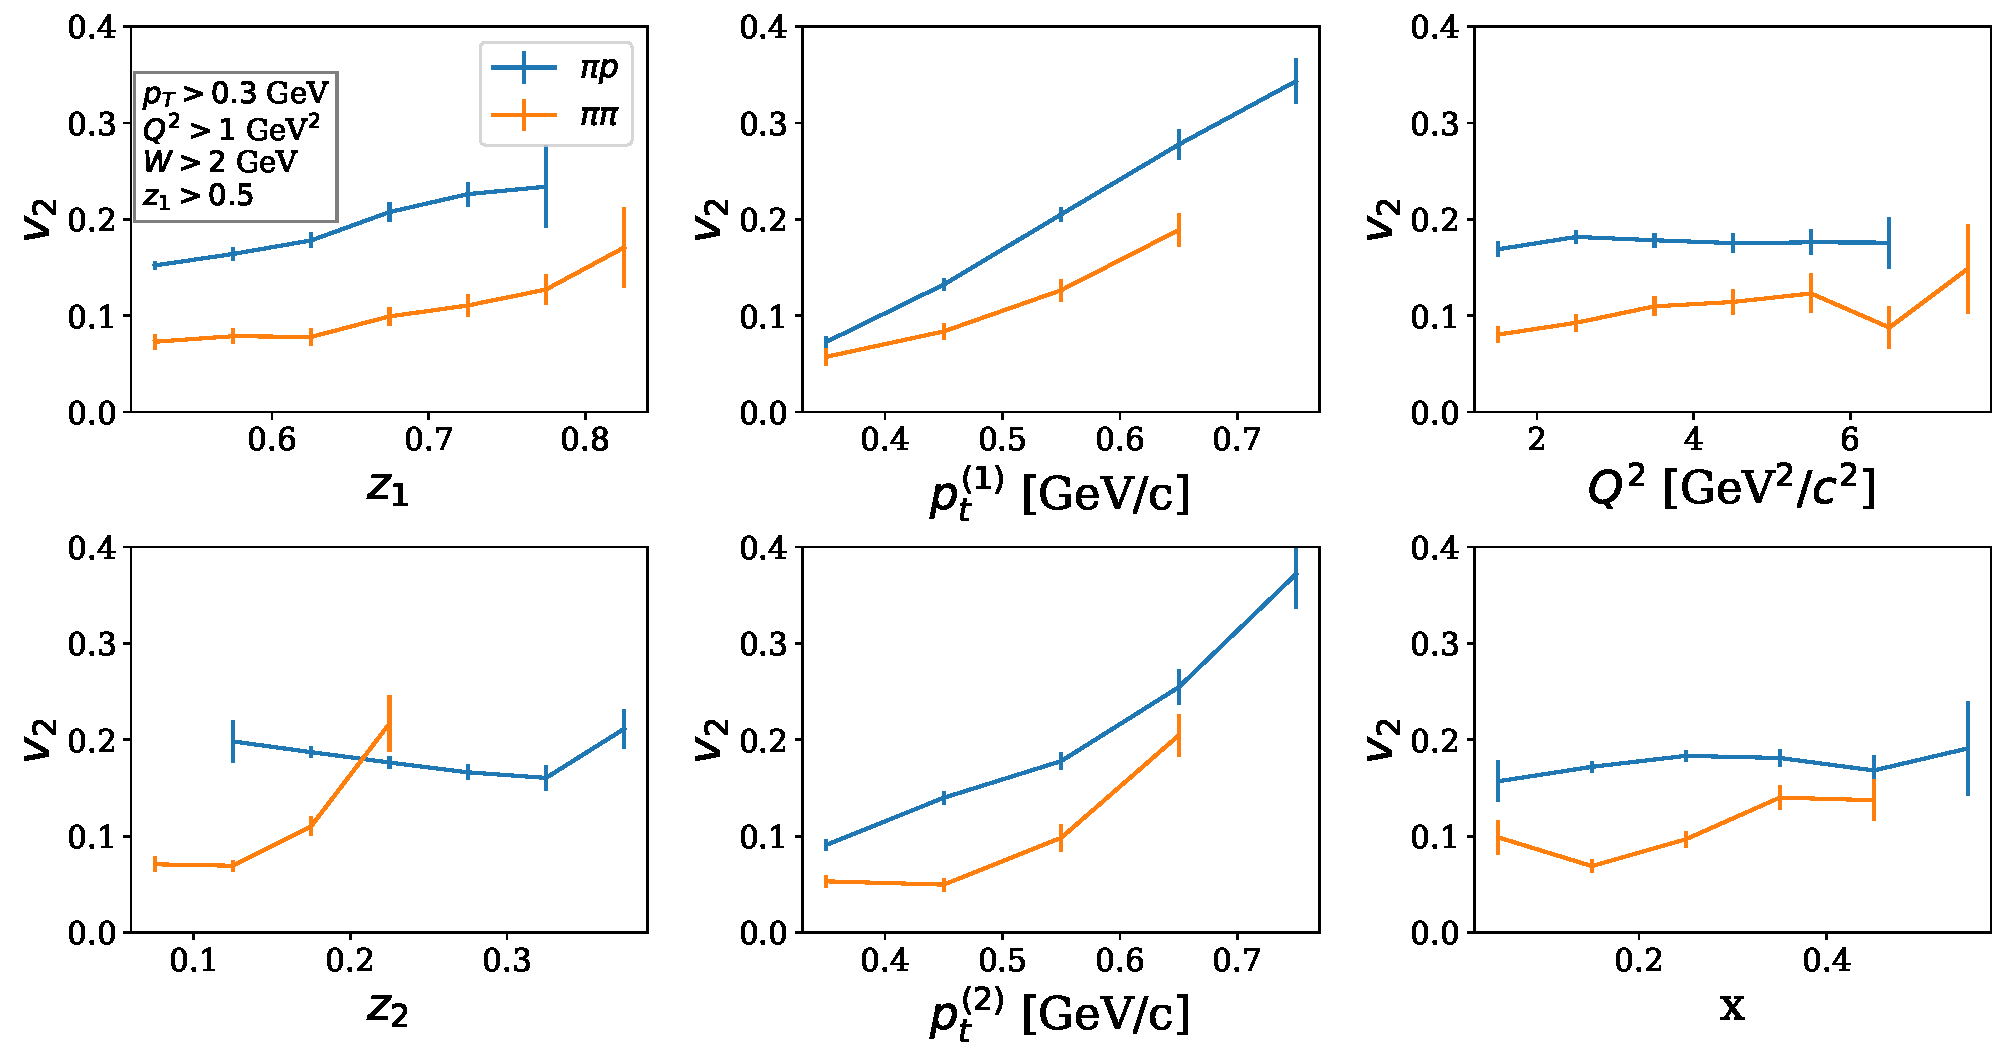
\includegraphics[width=\textwidth]{v2_vs_stuff1.pdf}
    \caption{$v_2$ vs several kinematic variables: $z_1$, $z_2$, etc.}
    \label{fig:v2_vs_stuff}
\end{figure}

The upper limits in the ridge-yield analysis are shown in Fig.~\ref{fig:money_plot} as functions of the track multiplicity, and are compared to results from CMS \cite{Khachatryan:2010gv,CMS:2012qk,Khachatryan:2015lva}, HERA and ALEPH \cite{Lee:2019tmr}.  The correlation functions within each bin in track multiplicity are shown in Fig.~\ref{fig:corrs_vs_ntracks}.  In these plots, we define the track multiplicity to include only \textit{hadronic} tracks passing the cuts in Sec.~\ref{sec:hadron_selection}.  

\begin{figure}
    \centering
    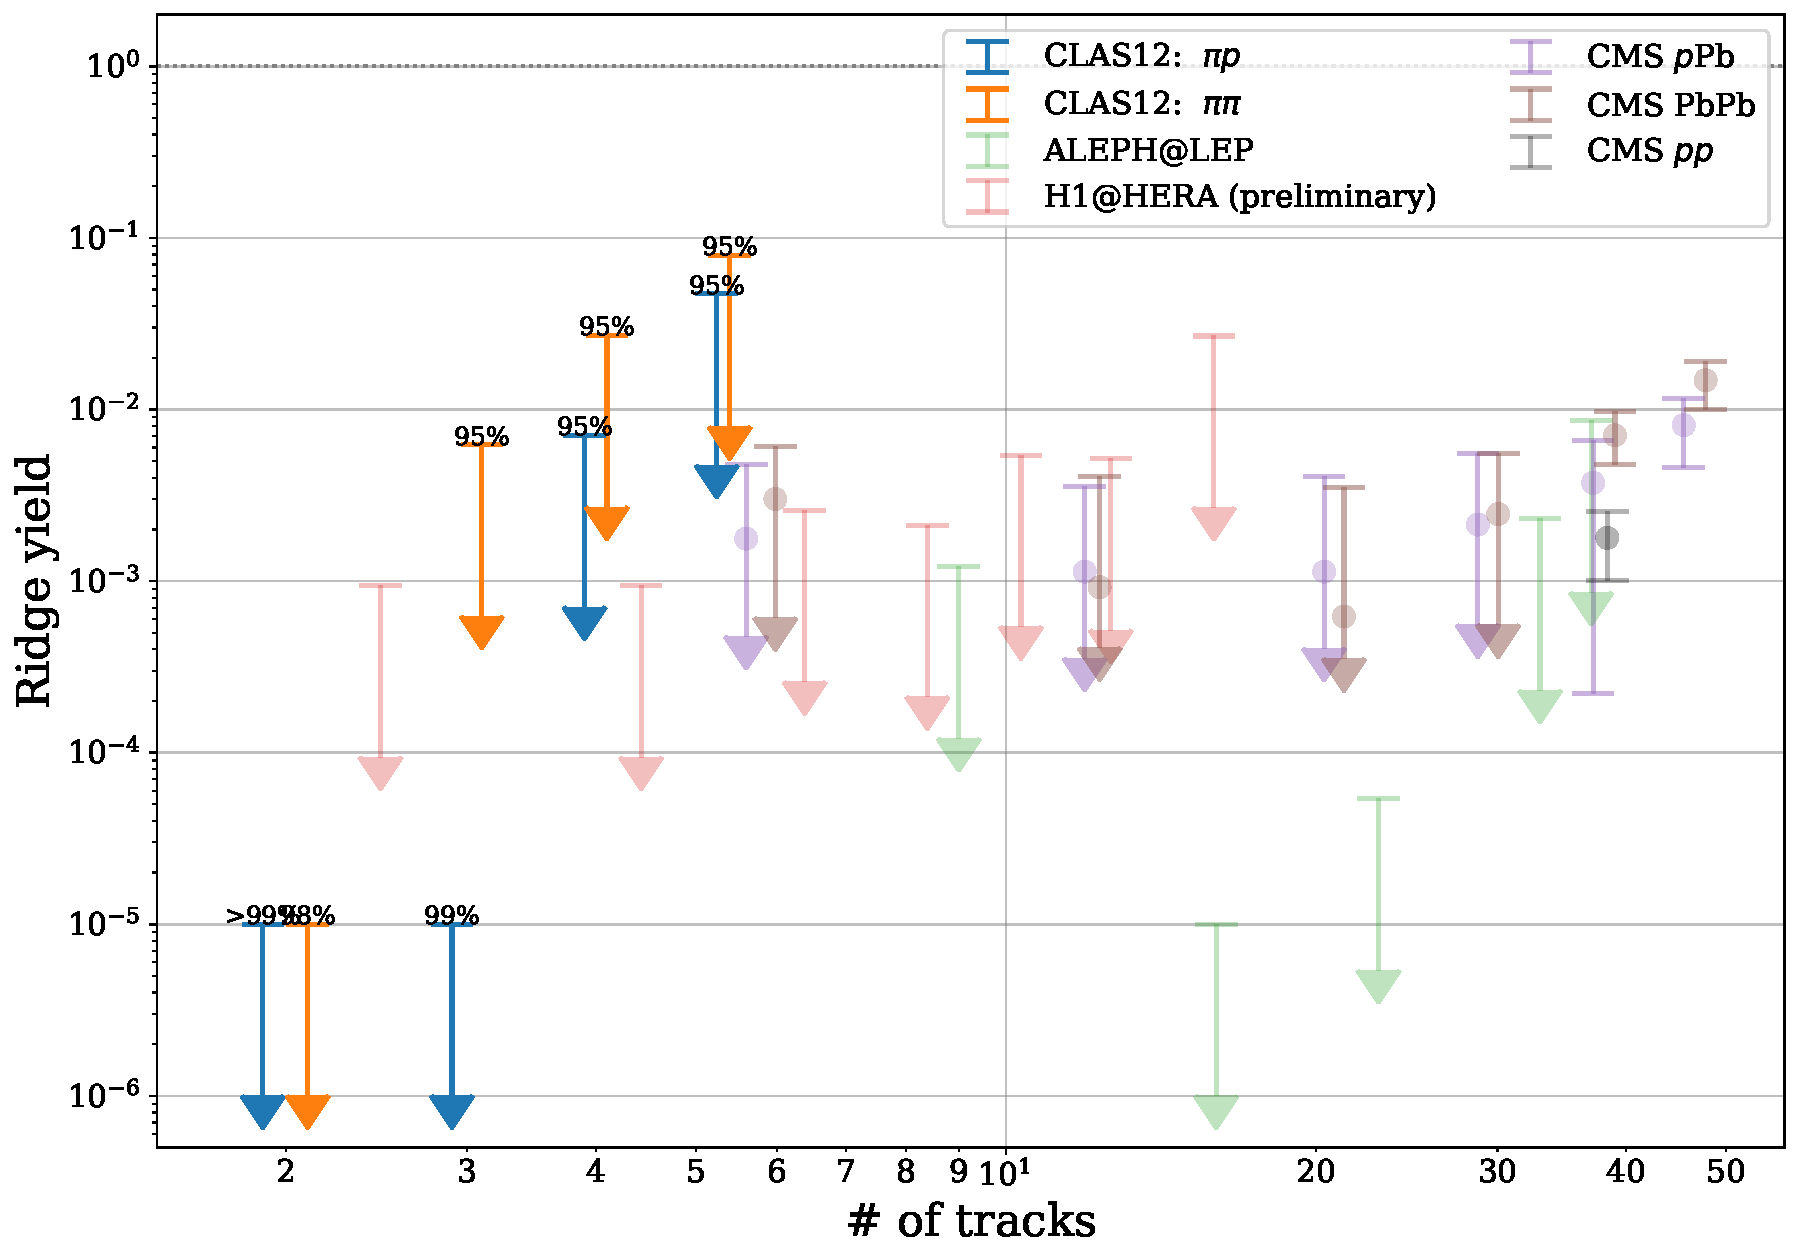
\includegraphics[width=\textwidth]{moneyplot.pdf}
    \caption{Upper limits from ridge-yield analysis in CLAS12, as functions of the track multiplicity.  Superimposed are the results from CMS \cite{Khachatryan:2010gv,CMS:2012qk,Khachatryan:2015lva}, HERA, and ALEPH \cite{Lee:2019tmr}}
    \label{fig:money_plot}
\end{figure}

\begin{figure}
    \centering
    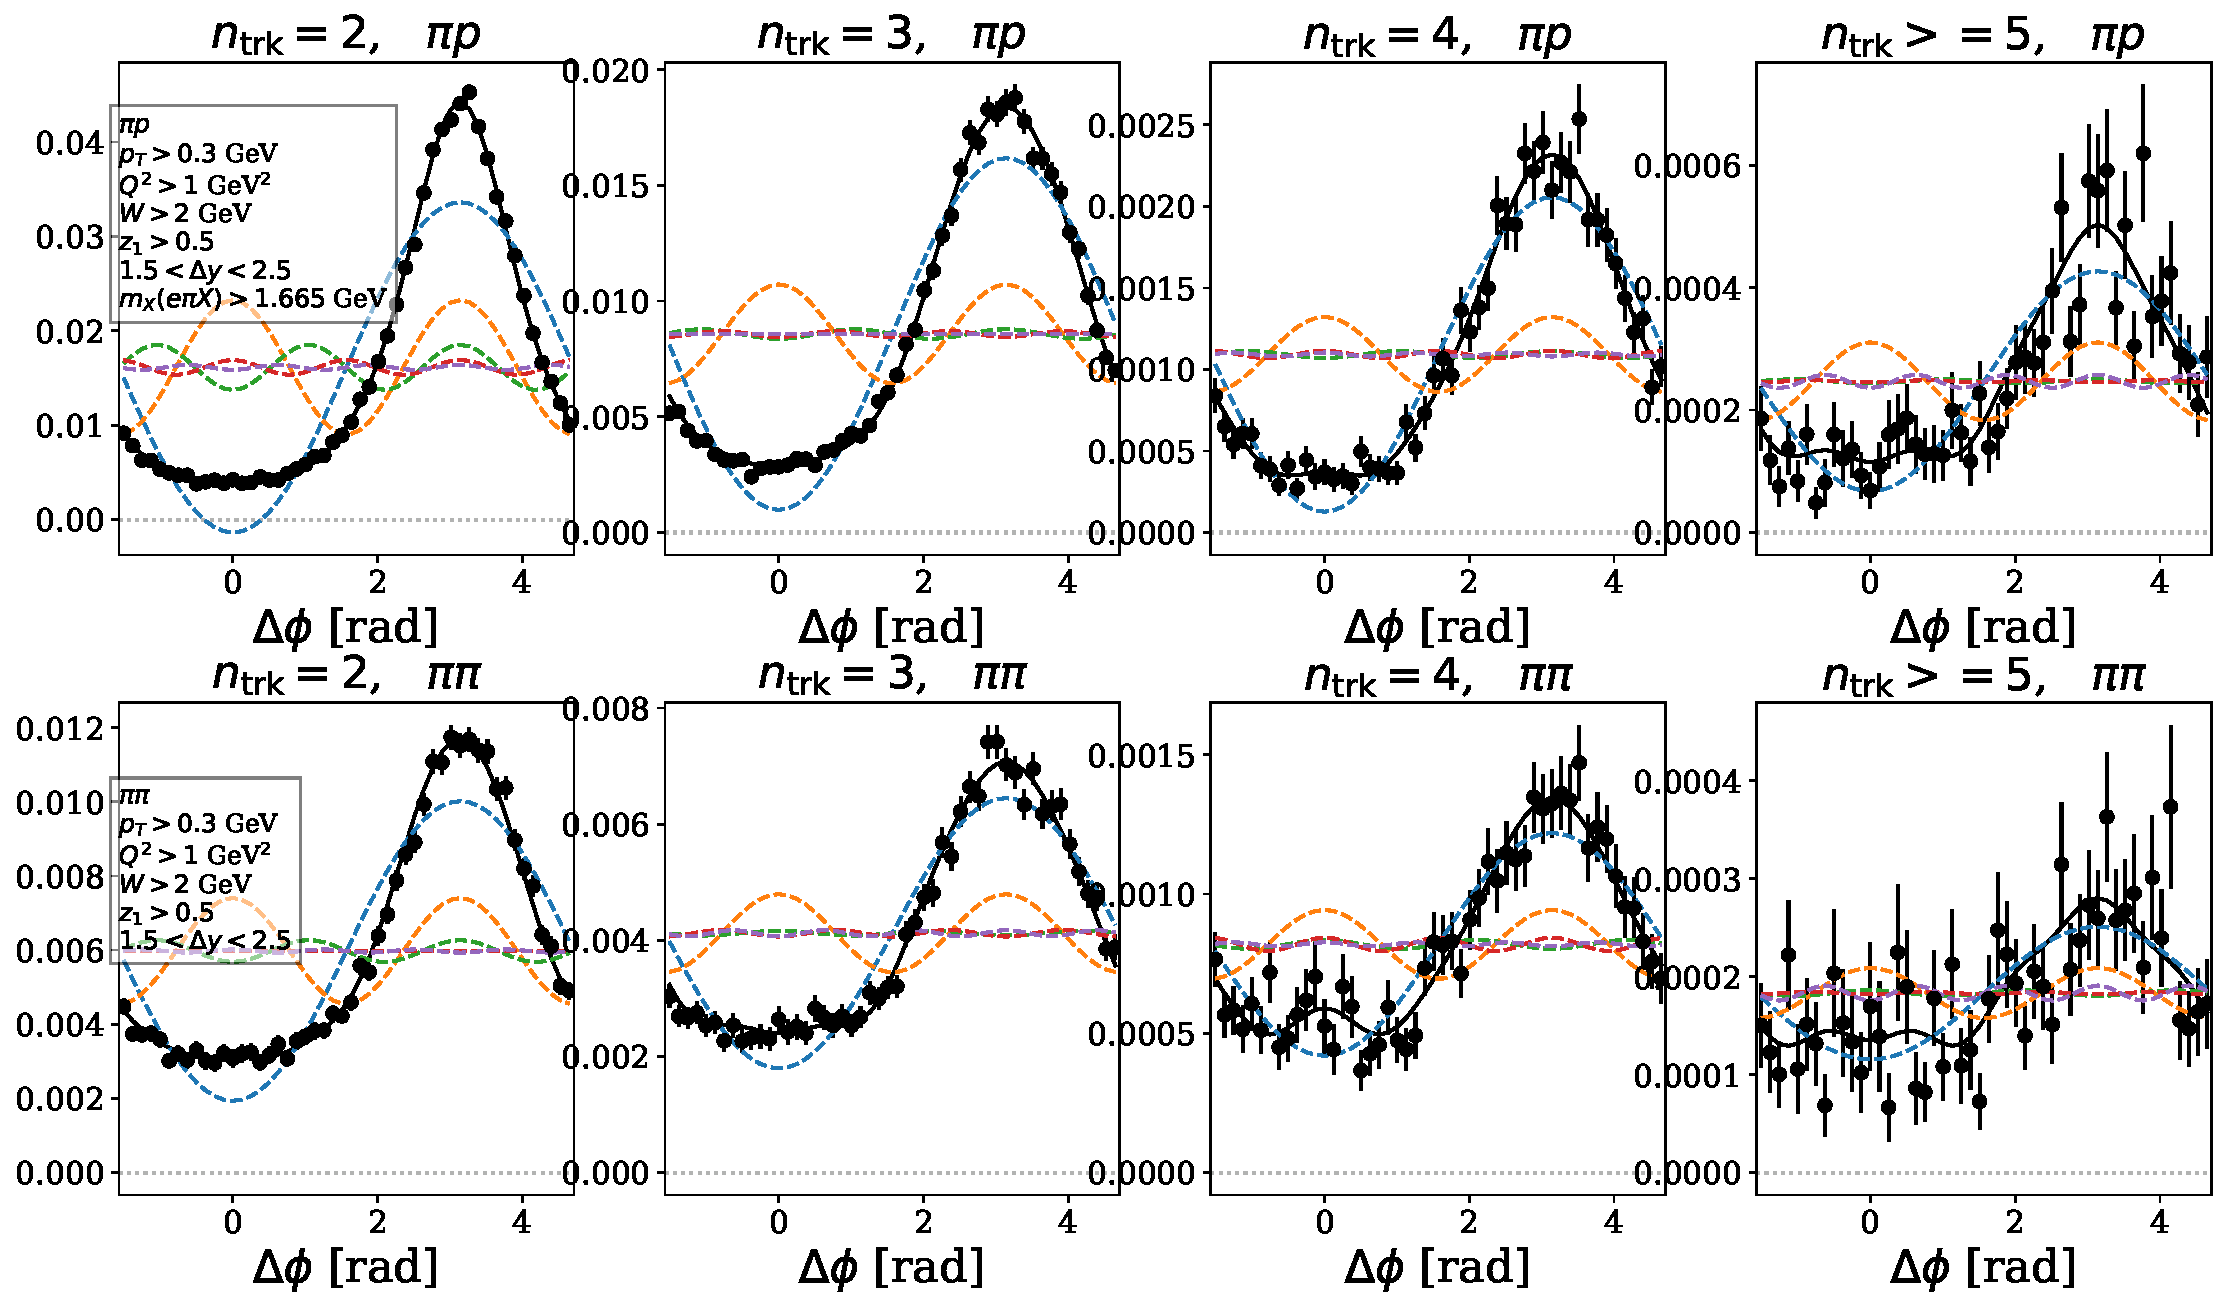
\includegraphics[width=\textwidth]{corrs_vs_ntracks.pdf}
    \caption{Correlation functions for different track-multiplicity bins, for $\pi p$ (top) and $\pi\pi$ events.  These are the same bins used in Fig~\ref{fig:money_plot}.}
    \label{fig:corrs_vs_ntracks}
\end{figure}
\section{Conclusions} \label{sec:conclusions}



\FloatBarrier
%\newpage
 \begin{appendices}
 \appendix
 %\input{Reproducibility}
 \end{appendices}
\FloatBarrier


\renewcommand\refname{Bibliography}
\bibliographystyle{unsrt} % or try abbrvnat or unsrtnat
\bibliography{biblio} % refers to example.bib


\end{document}

